\documentclass[xcolor=svgnames,xcolor=table,aspectratio=169]{beamer}
\usetheme{Boadilla}

\usepackage[utf8]{inputenc}
\usepackage[T1]{fontenc}
\usepackage{lmodern}
\usepackage{sourcecodepro}
\usepackage[whole]{bxcjkjatype}
\usepackage[backend=biber]{biblatex}
\addbibresource{slides.bib}
\usepackage{listings}
\lstset{
  language={},
  basicstyle=\footnotesize,
  keywordstyle=\color{blue},
  morekeywords={classdef,endclassdef,properties,endproperties,methods,endmethods},
}
\usepackage{mathtools}
\usepackage{multimedia}
\usepackage{multirow}
\usepackage{siunitx}
\usepackage{pifont}
\usepackage{tikz}
\newcommand*\colorcheck[1]{%
  \expandafter\newcommand\csname #1check\endcsname{\textcolor{#1}{\ding{52}}}%
}
\usepackage{fix-cm}
\newcommand{\regmark}{\textsuperscript{\tiny\textregistered}}

\colorcheck{green}

\title[Numerical verification in high-level languages]
  {More system independent usage of numerical verification algorithms
  written in high-level programming languages}
\author[Kai T. Ohlhus]{OHLHUS, Kai Torben}
\institute[TWCU]{
  Graduate School of Science \\
  Tokyo Woman's Christian University}
\date[January 30, 2020]{Workshop on Large-scale Parallel Numerical Computing Technology (LSPANC) \\
RIKEN Center for Computational Science (R-CCS), Kobe, Japan \\[1em]
January 29 -- 30, 2020
}


\begin{document}
\renewcommand*{\arraystretch}{1.2}

\frame{\titlepage}
\frame{\tableofcontents}



\section{Introduction and system dependency problem}


\begin{frame}{Introduction}
\begin{itemize}
\itemsep1em
\item
\textbf{Verification methods / algorithms}:
\begin{itemize}
\itemsep1em
\item
"Mathematical theorems are formulated
whose assumptions are verified with the aid of a computer."
(Rump \cite{Rump2010})
\end{itemize}

\item
\textbf{High-level programming language}:
\begin{itemize}
\itemsep1em
\item
Providing abstractions (e.g. no data types, memory management)

\item
Less error prone, more expressive, faster development of algorithms.

\item
Compiled or interpreted.

\item
Not necessarily limited or slow.
Depending on the purpose / computation.

\item
\textbf{But:} Code / tools / libraries providing the abstraction become dependencies.
\end{itemize}
\end{itemize}
\end{frame}




\begin{frame}{Introduction}
\begin{itemize}
\itemsep1em
\item
In my PhD thesis and before \cite{Ohlhus2019,Chaykin2016} we computed
rigorous error bounds for \textbf{conic linear programs} with up to
\textbf{19 million variables and 27 thousand constraints}.

\item
The following simplified software stack (mostly high-level, interpreted code)
was used\footnote{\url{https://vsdp.github.io/}}:
\end{itemize}
\begin{columns}
\begin{column}{0.05\textwidth}
\end{column}
\begin{column}{0.45\textwidth}
\includegraphics[width=\textwidth]{res/vsdp_workflow}
\end{column}
\begin{column}{0.45\textwidth}\tiny
\begin{tabular}{|c|c|}
\hline
\multicolumn{2}{|c|}{\cellcolor{orange!20}VSDP} \\
\hline
\cellcolor{orange!20}INTLAB
& \cellcolor{red!20}CSDP / MOSEK / SDPA / SeDuMi / SDPT3, ... \\
\hline
\multicolumn{2}{|c|}{Matlab / GNU Octave} \\
\hline
\multicolumn{2}{|c|}{"Linux"} \\
\hline
\end{tabular}
\end{column}
\end{columns}
\begin{itemize}
\itemsep1em
\item
For larger problem instances the current "Linux" system was insufficient.

$\rightarrow$ Move to another "Linux" system, but...
\end{itemize}
\end{frame}



\begin{frame}{There is not just "Linux"...}

\begin{table}
\begin{tabular}{cccc||ccc}
First release & Distribution     & Kernel
& GCC\footnote{MATLAB\regmark requires GCC 6.3
\url{https://www.mathworks.com/support/requirements/supported-compilers.html}}
& Scilab & Octave & ... \\
& & 5.5 & 9.2 & 6.0.2 & 5.1 & \\
\hline
2019          & RHEL/CentOS 8.1  & 4.18   & 8.3 &  -    &  -  & \\
2018          & SLES 15.1        & 4.12   & 7.2 &  -    &  -  & \\
2018          & Ubuntu 18.04.3   & 4.15   & 7.3 & 6.0.1 & 4.2 & \\
2016          & Ubuntu 16.04.6   & 4.4    & 5.4 & 5.5   & 4.0 & \\
2014          & SLES 12.4        & 4.12   & 4.8 &  -    &  -  & \\
2014          & RHEL/CentOS 7.7  & 3.10   & 4.8 &  -    & 3.8 & \\
2010          & RHEL/CentOS 6.10 & 2.6
& 4.4\footnote{No C11/C++11 support
\url{https://gcc.gnu.org/projects/cxx-status.html}}
& - & 3.4 \\
\end{tabular}
\end{table}

\end{frame}



\begin{frame}{What to expect from "Linux-clusters" today?}
\begin{itemize}
\itemsep1em
\item
Many \textbf{free and open source} high-level programming languages
and libraries (e.g. Scilab, Octave, OpenBLAS, ...)
are not suitable/not good performing:
\begin{itemize}
\item
outdated versions or missing
\begin{itemize}
\item
system dependent approaches (packages)

$\quad$(RedHat: devtoolsets, EPEL, ...; Ubuntu Backports)

\item
system independent approaches

$\quad$(Anaconda [Python], flatpak, snap, ...)
\end{itemize}
\item
configured for general purpose systems
\begin{itemize}
\item
linked against reference implementations
\end{itemize}
\end{itemize}
\item
Mostly \textbf{proprietary} pendants
(e.g. MATLAB\regmark, CUDA\regmark, Intel\regmark MKL, ...)
are available in \textbf{more recent versions} on these "old" systems.

\item
Compiling missing software from source?
\begin{itemize}
\item
Dependencies often outdated too.
In case of Octave: OpenBLAS, SuiteSparse, Arpack, ...

\item
Space quotas, installation permissions, ...
\end{itemize}

\item
\textbf{Reproducibility} of previous results?
\end{itemize}
\end{frame}


\begin{frame}[fragile]{Sometimes things are even worse...}
\begin{itemize}
\item
Kashiwagi described a problem\footnote{\url{http://verifiedby.me/adiary/060}}
for Linux + OpenBLAS ({\color{DarkRed}multiple threads}) + Octave
and switching of the directed rounding mode.
It occurs in the following short example:
\end{itemize}

\begin{lstlisting}[language=Octave,xleftmargin=5em]
N = 5000;
A = rand(N);      % create random 5000x5000 matrix
B = rand(N);      %        elements in (0,1)
setround(-1);     % rounding downwards mode
C1 = A * B;       % lower bound for A*B
setround(+1);     % rounding upwards mode
C2 = A * B;       % upper bound for A*B
min(min(C2 - C1)) % should not be zero!
\end{lstlisting}

\begin{itemize}
\item
The default OpenBLAS package of most Linux distributions is compiled using
{\color{DarkRed}\texttt{CONSISTENT\_FPCSR=0}}, which means that the
\textbf{floating-point control and status register}
is not synchronized within multiple threads.

\item
{\color{DarkRed}
The software stack relies on a \textbf{version} and a \textbf{configuration}.}
\end{itemize}
\end{frame}




\begin{frame}{How to ensure complicated software stacks?}
\begin{columns}
\begin{column}{.3\textwidth}
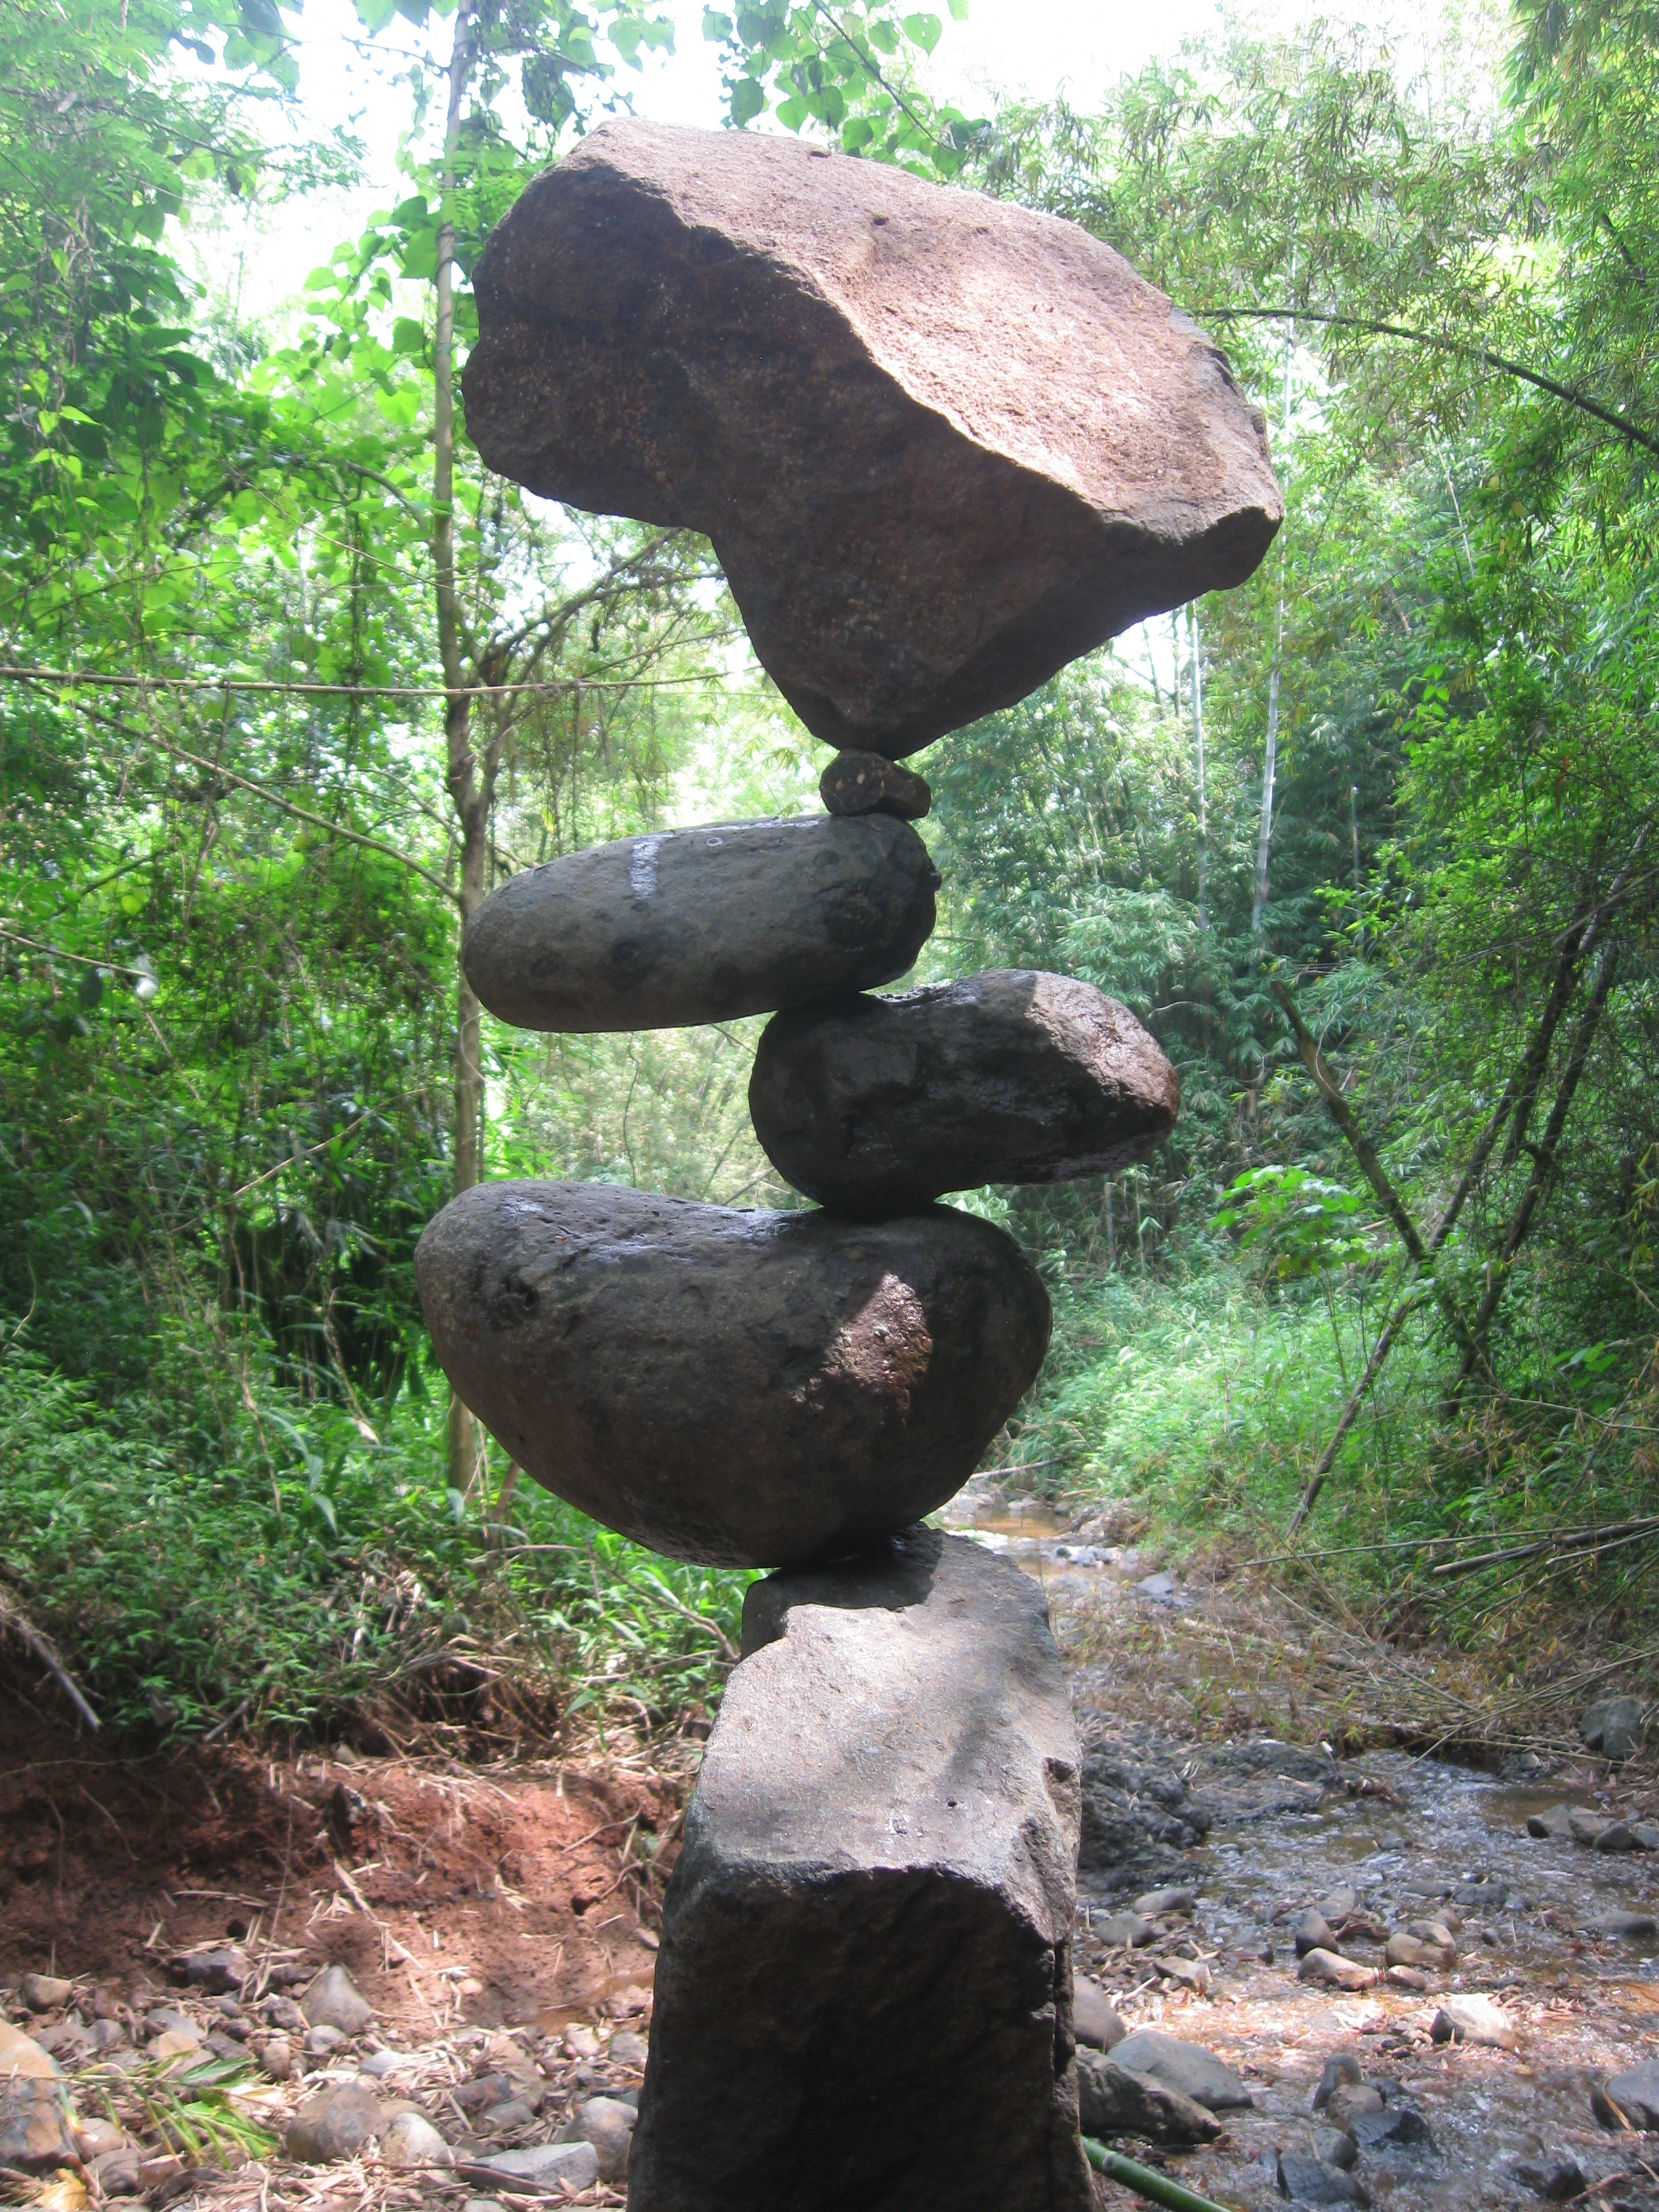
\includegraphics[width=\textwidth]{res/rock_balancing.jpg}
\end{column}
\begin{column}{.65\textwidth}
\begin{center}
\begin{tabular}{|c|c|}
\hline
\multicolumn{2}{|c|}{VSDP{\color{red}@2018}} \\
\hline
\multirow{3}{*}{INTLAB{\color{red}@11}}
& CSDP{\color{red}@6.2.0} / MOSEK{\color{red}@8.1.0.62} / \\
& SDPA{\color{red}@7.3.8} / SeDuMi{\color{red}@1.32} / \\
& SDPT3{\color{red}@4.0}, ... \\
\hline
\multicolumn{2}{|c|}{GNU Octave{\color{red}@4.4.1}} \\
\multicolumn{2}{|c|}{{\color{blue}linked against}
OpenBLAS{\color{red}@0.3.7}} \\
\multicolumn{2}{|c|}{{\color{blue}configured with}
{\color{DarkGreen}\texttt{CONSISTENT\_FPCSR=1}}} \\
\multicolumn{2}{|c|}{...} \\
\hline
\end{tabular}
\end{center}

\begin{itemize}
\itemsep1em
\item
Similar problem investigated by Shudler et al. \cite{Shudler2019}
for SENSEI, presented on SC'19 in Denver.
\end{itemize}
\end{column}
\end{columns}
\vfill
{\tiny Image:
\url{https://commons.wikimedia.org/wiki/File:Rock_balancing_(Counter_Balance).jpg}
}
\end{frame}



\section{Solution 1: Spack}
\frame{\tableofcontents[currentsection]}



\begin{frame}{\textbf{S}upercomputing \textbf{pack}age
manager\footnote{\url{https://spack.io} and \cite{Gamblin2015}.} (1/5)}

\begin{itemize}
\itemsep1em
\item
Very actively developed since 2013
(started by members of the Lawrence Livermore National Laboratory).

\item
Contains currently 3838 packages (812 Python, 782 R).

\item
Addresses several problems with current Linux software distribution models:
\begin{itemize}
\itemsep1em
\item
Packages and (some!) dependencies are build from source. ($\neq$ ArchLinux).

\item
Define target architecture, compiler (incl. icc), version,
configuration (variants), ...

\textbf{$\rightarrow$ Reproducibility!}

\item
Packages \textbf{peacefully coexist} on the same machine.

\textbf{$\rightarrow$ Maintenance!}
\end{itemize}

\item
Will be the default package manager for
Fugaku\footnote{\url{https://postk-web.r-ccs.riken.jp/oss/public/}}.
\end{itemize}
\end{frame}



\begin{frame}[fragile]{Spack (2/5)}

\texttt{{\color{blue}\$ spack info} openblas}

\begin{lstlisting}[escapeinside={\%}{\%}]
Safe %{\tt\color{red}versions}%:
    %{\tt\color{red}0.3.7}%      https://github.com/xianyi/OpenBLAS/archive/v0.3.7.tar.gz
...
%{\tt\color{DarkGreen}Variants:}%
    Name [Default]    Allowed values          Description
    ==============    ====================    ==============================

    %{\tt\color{DarkGreen}ilp64}% [off]       True, False             Force 64-bit Fortran native
                                              integers
    pic [on]          True, False             Build position independent
                                              code
    shared [on]       True, False             Build shared libraries
    %{\tt\color{DarkGreen}threads}% [none]    pthreads, openmp,       Multithreading support
                      none
\end{lstlisting}

\texttt{{\color{blue}\$ spack install}
octave{\color{red}@5.1.0}
\^{}openblas{\color{red}@0.3.7}{\color{DarkGreen}+ilp64 threads=openmp}}

\hfill{\color{DarkGreen}CONSISTENT\_FPCSR=1}
\end{frame}



\begin{frame}{Spack (3/5)}
\begin{itemize}
\item
Spack grammar in extended Backus-Naur form \cite{Gamblin2015}:
\end{itemize}
\begin{center}
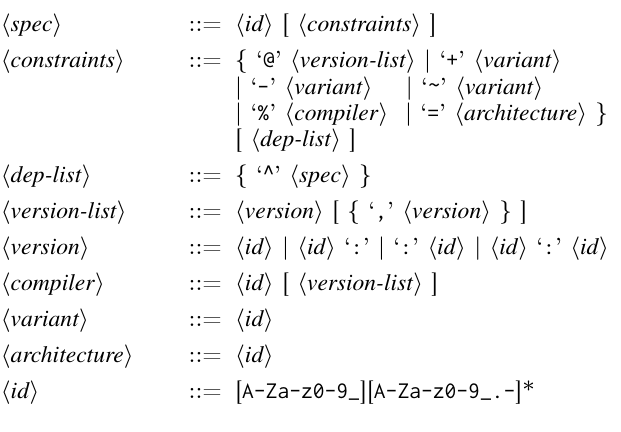
\includegraphics[width=0.6\textwidth]{res/spack-grammar}
\end{center}
\end{frame}



\begin{frame}{Spack (4/5)}
\begin{itemize}
\item
Example Spack package definition written in Python \cite{Gamblin2015}:
\end{itemize}
\begin{center}
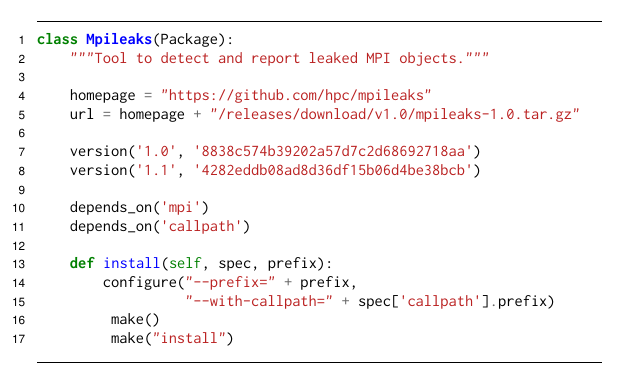
\includegraphics[width=0.7\textwidth]{res/spack-spec}
\end{center}
\end{frame}



\begin{frame}{Spack (5/5) summary}
\begin{itemize}
\item
Spack allows to obtain more customized packages
than classical Linux package managers.

\item
It addresses the resulting combinatorial configuration space
by building only requested combinations.

\item
Build receipts are maintained and tested by several HPC facilities.
\end{itemize}
\begin{center}
\includegraphics[width=0.5\textwidth]{res/spack-combinatoric}
\end{center}
\end{frame}



\section{Solution 2: Singularity}
\frame{\tableofcontents[currentsection]}



\begin{frame}{Singularity \cite{Kurtzer2017} - Container for HPC?}
\begin{itemize}
\itemsep1em
\item
Initial version created by Gregory M. Kurtzer about 2015
at the Berkeley National Lab.

\item
Still free software developed by Sylabs Inc.

\item
\textbf{Lightweight} container solution:

\begin{itemize}
\itemsep1em
\item
Container overhead negligible
\cite{Herbein2016,Le2017,Younge2017,Shudler2019}.

\item
Singularity images are a single self-contained file.
Distribution by copy\&paste, no DockerHub, ...

\item
Native MPI, Ininiband, and GPU support.

\item
No root daemon for the execution of Singularity images necessary.
Runs with the privileges of the user.
$\rightarrow$ Security.
\end{itemize}
\end{itemize}
\end{frame}



\begin{frame}[fragile]{Singularity definition files (1/3)}
\begin{lstlisting}[xleftmargin=5em,language=Bash]
Bootstrap: docker
From: centos

%post

    # Install some development tools to build our code
    yum install -y \
      cmake \
      environment-modules \
      gcc-gfortran \
      gnuplot \
      python3 \
      texinfo \
      wget
\end{lstlisting}
\end{frame}



\begin{frame}[fragile]{Singularity definition files (2/3)}
\begin{lstlisting}[xleftmargin=5em,language=Bash]
%post
    ...

    # Setup Spack
    cd /
    wget https://github.com/spack/spack/archive/develop.tar.gz
    tar -xf develop.tar.gz
    mv spack-develop spack
    source /spack/share/spack/setup-env.sh

    spack install octave@5.1.0 \
      ^ openblas@0.3.7+ilp64 threads=openmp \
                             CONSISTENT_FPCSR=1

    # Tidy up, shrink container size ~710 MB --> ~590 MB
    
    rm -Rf /develop.tar.gz /spack/var/spack/cache/
    yum clean all
\end{lstlisting}
\end{frame}



\begin{frame}[fragile]{Singularity definition files (3/3)}
\begin{lstlisting}[xleftmargin=5em,language=Bash]
%runscript

    # Commands to be executed, when container starts
    spack load octave
    octave

%environment

    export LC_ALL=en_US.UTF-8
    source /usr/share/Modules/init/sh
    source /spack/share/spack/setup-env.sh
\end{lstlisting}
\end{frame}



\begin{frame}[fragile]{Build and run Singularity Image Files (SIF)}
\begin{itemize}
\itemsep1em
\item
Build SIF with root privileges

\texttt{\color{blue}sudo singularity build octave.sif octave.def}

\begin{itemize}
\itemsep1em
\item
Reduce image size, avoid unnecessary tools.

\item
Reduce build time, trade-off install via Spack or guest Linux package manager.

\texttt{yum} in this case.
\end{itemize}

\item
Run with user privileges

\texttt{\color{blue}singularity run octave.sif}

\begin{itemize}
\itemsep1em
\item
Access to user's \texttt{/home} directory.

\item
Other host system directories by default not accessible,
but "\verb|--bind|" possible.
\end{itemize}
\end{itemize}
\end{frame}



\section{Summary and future work}



\begin{frame}
\begin{itemize}
\itemsep2em
\item
Summary
\begin{itemize}
\itemsep1em
\item
High-level programming languages provide useful abstractions for faster
and less error prone development of verification methods.

\item
To provide these abstractions sometimes nontrivial software stacks are required.

\item
Spack can be used to uniquely specify and build these software stacks
more independent of the underlying Linux distribution.

\item
Singularity containers further increase independence of the underlying system
without sacrificing security, InfiniBand, MPI, or CUDA support.
\end{itemize}

\item
Future work
\begin{itemize}
\itemsep1em
\item
Improve Spack receipts to support all required variations for VSDP.

\item
More performance tests with Singularity containers
and large scale linear conic programs.
\end{itemize}
\end{itemize}
\end{frame}



\begin{frame}
\begin{center}
\textbf{\Large Thank you for your attention!}
\bigskip

\bigskip

\textbf{\Large Questions?}
\vfill
\end{center}
\end{frame}



% Backup slides.
\newcounter{finalframe}
\setcounter{finalframe}{\value{framenumber}}



\begin{frame}[allowframebreaks]
\printbibliography
\end{frame}



\setcounter{framenumber}{\value{finalframe}}

\end{document}
